% \documentclass[landscape,a0b,final]{a0poster}
\documentclass[portrait,a0b,final,a4resizeable]{a0poster}

%%% Option "a4resizeable" makes it possible ot resize the
% poster by the command: psresize -pa4 poster.ps poster-a4.ps
% For final printing, please remove option "a4resizeable" !!
% \usepackage[a0paper]{geometry}
\usepackage[dvips]{graphicx}
\usepackage{epsfig}
\usepackage{color}
\usepackage{shadow}
\usepackage{multicol}
% \usepackage{times}

% \usepackage{showframe} 

% \usepackage{pstricks}
% \usepackage{algorithm}
% \usepackage{subfigure}}
% \usepackage{amsmath}
% \usepackage{amssymb}
% \usepackage{url}
\usepackage{sectsty}
\usepackage{definitions}
% \usepackage[absolute]{textpos}
\usepackage[it]{subfigure}
\usepackage{booktabs}
\usepackage{multirow}
\usepackage{setspace}
% \usepackage[scaled=0.8]{DejaVuSansMono}

%%% Size of Poster etc.
\newlength{\textArea}
\setlength{\textArea}{121cm}  % for a0b = A0-big !!
\setlength{\columnsep}{3cm}
\setlength{\columnseprule}{2mm}
\setlength{\parindent}{0.0cm}
% \usepackage[capitalise]{cleveref}

% \addtolength{\textwidth}{-4cm}
\usepackage{fontspec}
% \setmainfont[BoldFont={FiraSans-Bold.ttf}]{FiraSans-Light.ttf}
\usepackage[sfdefault]{FiraSans}

\RequirePackage{algorithmicx}
% \RequirePackage{algorithmic}
\usepackage[noend]{algpseudocode}
\RequirePackage{algorithm}
\newcommand*\Let[2]{\State #1 $\gets$ #2}

%%%%%%%%%%%%%%%%%%%%%%%%%%%%%%%%%%%%%%%%%%%%%%%%%%%%%%%%%%%%%%%%%%%%%%%%%%%%%%%% 
%%% Begin of Document
\renewcommand{\normalsize}{\large}
\usepackage[retainorgcmds]{IEEEtrantools}
\begin{document}
\bstctlcite{IEEEexample:BSTcontrol}
\definecolor{backgroundCol}{rgb}{1,1,1} % Cardiff yellow
\pagecolor{backgroundCol}

%%%%%%%%%%%%%%%%%%%%%%%%%%%%%%%%%%%%%%%% 
% Definition of Colors
% Background- and Text-color
% \definecolor{mainCol}{rgb}{0.91,0.91,1}
% \definecolor{TextCol}{rgb}{0,0,0}
% \definecolor{mainCol}{rgb}{0.839,0.212,0.2784}% 214 54 71
% \definecolor{mainCol}{rgb}{0.8549,0.2196,0.2824}% 214 54 71
\definecolor{mainCol}{rgb}{0.8078,0.0196,0.2235}% According to the website
\definecolor{TextCol}{rgb}{1,1,1}
\definecolor{black}{rgb}{0,0,0}

\setlength{\sboxrule}{2pt}
\setlength{\sboxsep}{0pt}

\vspace*{0cm}
%%% Title und Author
%%% University-emblem
% \shabox{%
  % \hfill
% \shabox{%
    \quad\!\begin{minipage}[c][11cm][c]{13cm}
      % \begin{center}
      \vspace{1cm}
      
\includegraphics[width=11cm]{cu}
      \nobreak
      % \end{center}
    \end{minipage}
  \colorbox{white}{
    \begin{minipage}[c][11cm][c]{51cm}
      \begin{center}{\fontspec{TruenoRg}
        \textcolor{mainCol}{
          {\VeryHuge TOWARDS DRIVERLESS RACING}}\\[1ex]
            \small Daniel Harbourne, Mohamed Binesmael, Molly Ragonnet, Matteo de Rosa,\\ Rachael Joyce,
    Deeon Roy, Ahmad Amer, Bryson Kwan, Kirill Sidorov}
      \end{center}
    \end{minipage}
  }
  % \colorbox{white}{
  % }
% \shabox{
\colorbox{white}{
    \begin{minipage}[c][11cm][c]{21cm}
      % \begin{center}
      \vspace{1cm}
      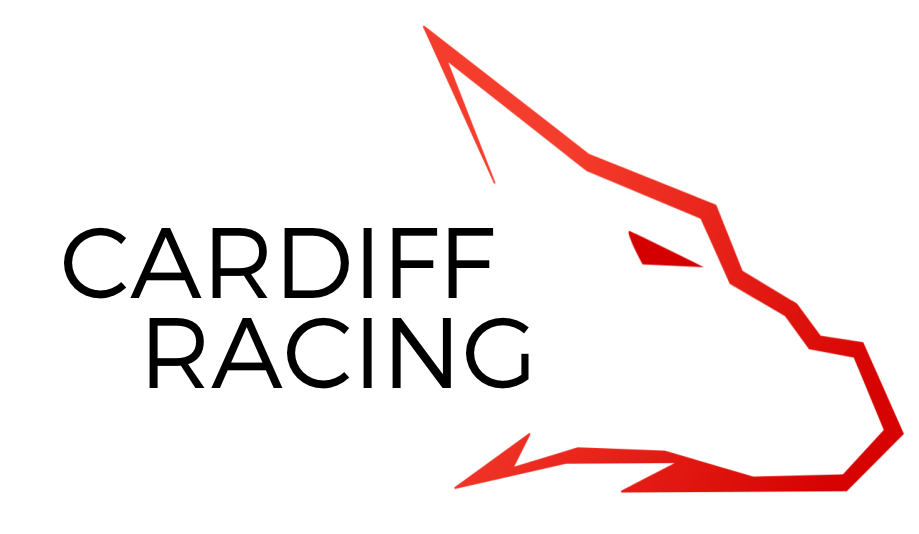
\includegraphics[width=21cm]{cr}
      \nobreak
      % \end{center}
    \end{minipage}
  }
% }
    % \hfill
%%% University-emblem
% }%\vspace{2cm}
\vspace{2cm}


%%% Begin of Multicols-Enviroment
\begin{multicols}{4}


  %%% Introduction
  \mysection{System Overview}
  We present the current progress of the Cardiff Racing Driverless team
  towards an autonomous racing vehicle.
  
  \begin{figurehere}
  \centering
  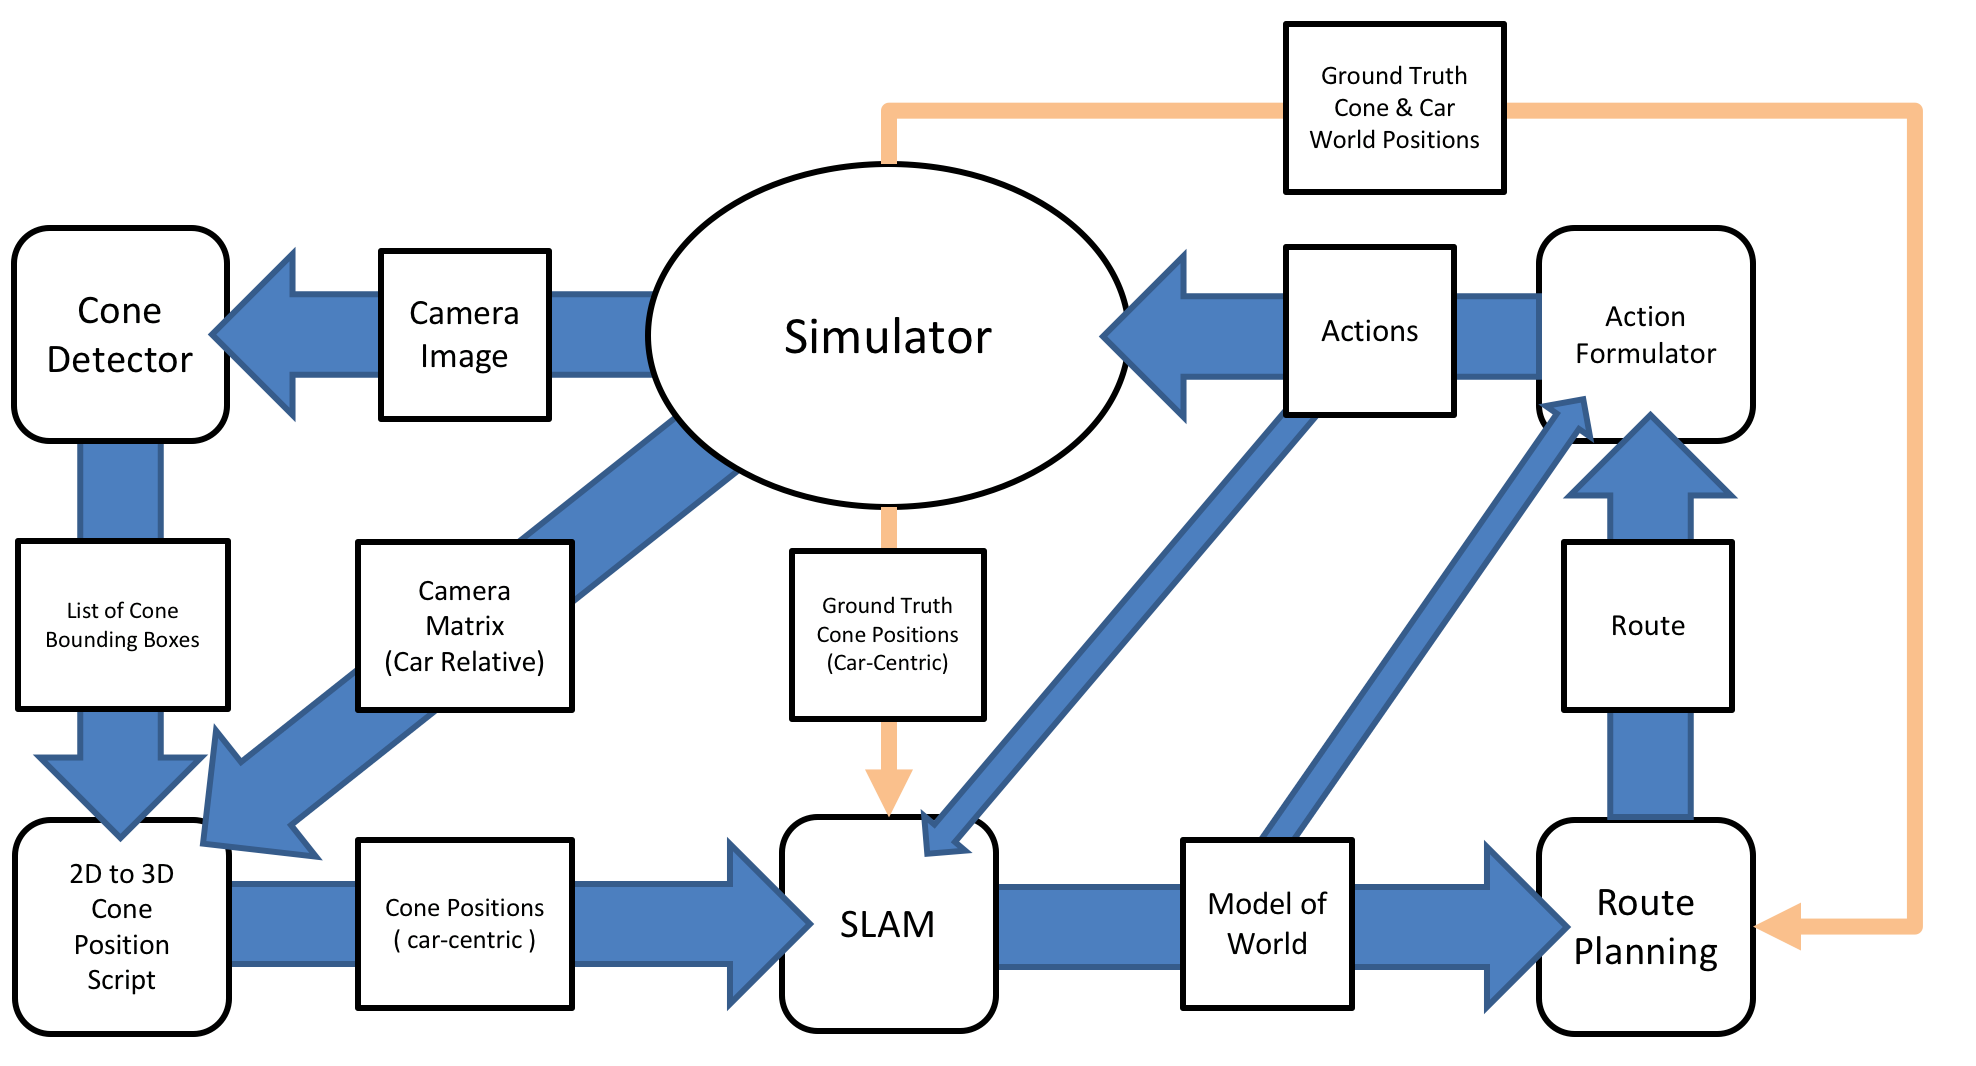
\includegraphics[width=1\linewidth]{img/system_new}
  \mycaption{System overview.}
  \label{fig:system}
\end{figurehere}
\begin{itemize}
\item Modular system architecture.
  \item Simulator in the loop.
\end{itemize}
\mysection{Cone Detection}
Three approaches tested:
\begin{itemize}
\item Viola-Jones cascade detector~\cite{viola01} with 3 features (LBP, Haar, HOG)
\item RCNN~\cite{girshick13}
  \item Fast-RCNN~\cite{girshick15}\\[1ex]
\end{itemize}

\begin{tablehere}
  \hfill\begin{tabular}{lll}
    \toprule
    &Images&Cones\\
    \midrule
    Training set & 988 & 2395\\
    Testing set& 100 & 711\\
    Total & 1088 & 3106\\
    \bottomrule
  \end{tabular}\hfill
  \mycaption{Cone dataset statistics.}
  \label{tab:dataset}
\end{tablehere}
A further 3219 negative images, including of race tracks, were used for
training.\\[1ex]

% \begin{tablehere}
%   \hfill
%   \small
%   \begin{tabular}{llrrr}
%     \toprule
%     Technique&Time, s&Precision&Recall&Avg. Prec.\\
%              \midrule
%     Haar&0.02863&0.8436&0.5007&0.4447\\
%     HOG&0.04459&0.8192&0.3952&0.3542\\
%     LBP&0.02715&0.8889&0.3601&0.3301\\
%     RCNN&4.44228&0.6986&0.3390&0.2797\\
%     Fast-RCNN&0.70334&0.2742&0.1674&0.0507\\
%     % Faster-RCNN&&&&\\
%     \bottomrule
%   \end{tabular}\hfill
%   \mycaption{Comparison of the cone detection techniques.}
%   \label{tab:cone}
% \end{tablehere}

\begin{tablehere}
  \hfill
  \small
  \begin{tabular}{llrrrr}
    \toprule
    Technique&{\Large$\tau$}&Time, s/im&Precision&Recall&Avg. Prec.\\
             \midrule
    Haar& 0.5&0.099&0.6297&0.6825&0.4493\\
    Haar& 0.3& &0.7901 &0.8564 &0.7287\\
    HOG& 0.5&0.165 &0.5122& 0.6217& 0.3781\\
    HOG& 0.3& & 0.8625 & 0.7581 & 0.5724\\
    LBP& 0.5&0.092 &0.5235 &0.6259 &0.3512\\
    LBP& 0.5& &0.6882 &0.8228 &0.6393\\
    RCNN& 0.5&4.442 &0.6777 &0.3727 &0.3052\\
    RCNN& 0.3& &0.8286 &0.4557 &0.4413\\
    Fast-RCNN& 0.5&0.703 &0.2742 &0.1674 &0.0507\\
    Fast-RCNN& 0.3& &0.5968& & 0.2583\\
    \bottomrule
  \end{tabular}\hfill
  \mycaption{Comparison of the cone detection techniques. {\Large$\tau$} is the IoU
    acceptance threshold between the detected and the ground truth bounding boxes.\\[0.5ex]}
  \label{tab:cone}
\end{tablehere}
Cascade detector performs better and faster than both deep learning techniques
in our experiments.\\[2ex]
\begin{minipage}{1.0\linewidth}
  \begin{figurehere}
    \label{fig:colour}
    \centering
    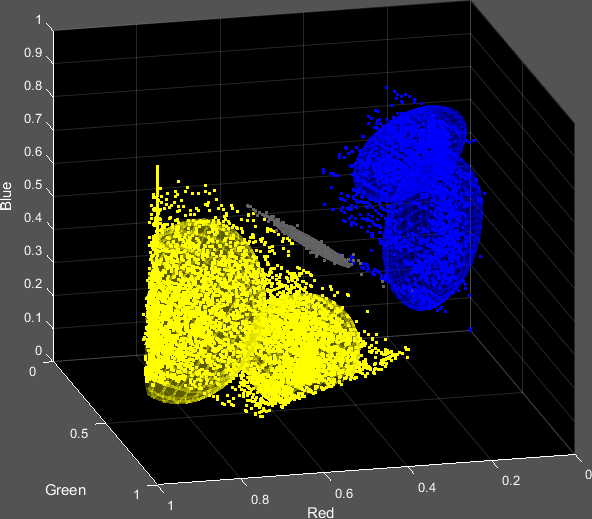
\includegraphics[width=0.49\linewidth]{img/colour_model_amz_rgb_3d}
    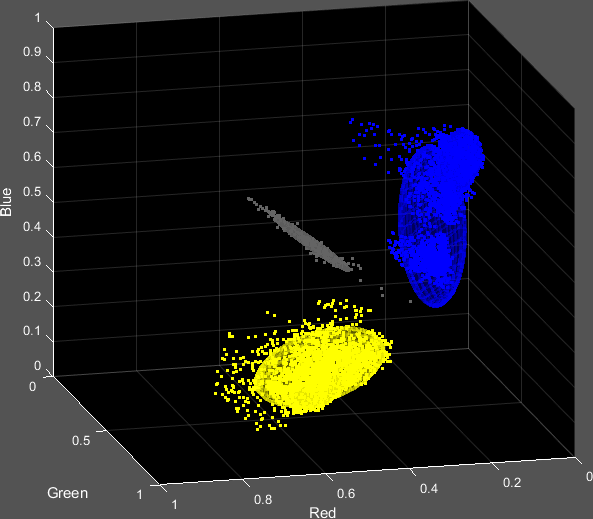
\includegraphics[width=0.49\linewidth]{img/colour_model_single_lap_rgb_3d}
    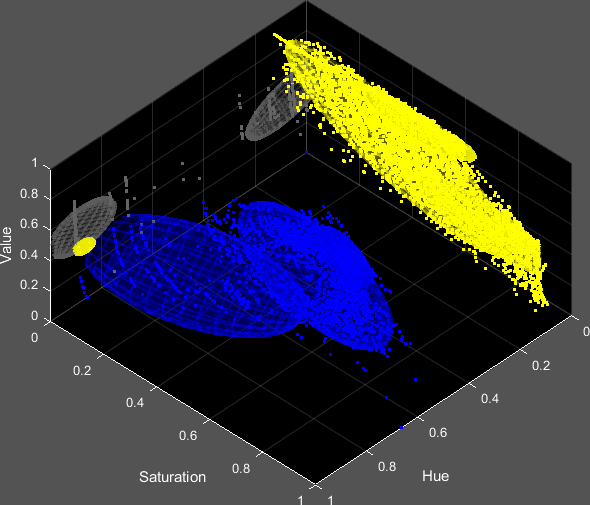
\includegraphics[width=0.49\linewidth]{img/colour_model_amz_hsv_3d}
    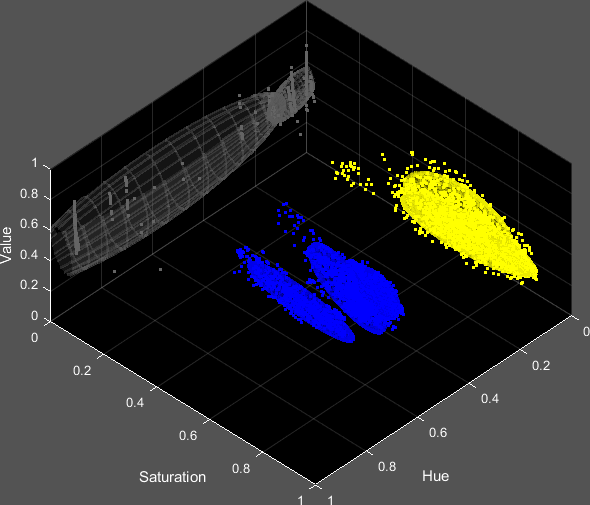
\includegraphics[width=0.49\linewidth]{img/colour_model_single_lap_hsv_3d}
    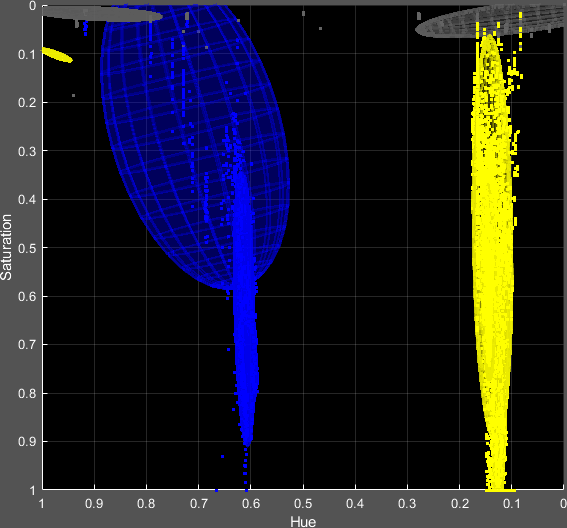
\includegraphics[width=0.49\linewidth]{img/colour_model_amz_hsv_2d}
    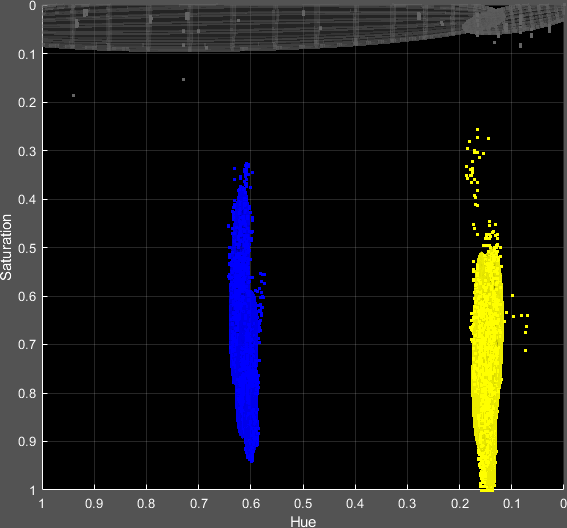
\includegraphics[width=0.49\linewidth]{img/colour_model_single_lap_hsv_2d}\\
    \qquad~~ AMZ data\qquad StreetDrone data \mycaption{Colour
      model. Ellipsoids delineate one standard deviation of the Gaussians in
      the mixture. \textsl{Top:} RGB space; \textsl{Middle and bottom:} HSV
      space.\label{fig:colour}}
  \end{figurehere}
\end{minipage}
A statistical model of colour (GMM) for
\begin{itemize}
\item Cone classification into blue/yellow
  \item Further filtering of false
    positives (see~Alg.~1
    and~Fig.~4)
    \item Invariance to illumination (HSV space and soft thresholding).
\end{itemize}
    
\begin{minipage}{1.0\linewidth}
  \begin{alghere}
    \small
    \myalgcaption{Filtering false-positives with colour model
      \label{alg:filter}}
    \begin{algorithmic}[1]
      \Require{Bounding box $W$, mixture models
        $(\vec{\mu}^b, \vec{C}^b)$,
    $(\vec{\mu^y}, \vec{C}^y)$ with $N_b$ and $N_y$ components, thresholds
$\tau_b$, $\tau_y$, $\rho_b$, $\rho_y$.}
      \State{$D^b\gets 0$, $D^y\gets 0$}
\For{\textrm{each
          pixel }$(r, g, b)\in W$}
      \Let{$\vec{x}=(h, s, v)$}{\Call{rgb2hsv}{$(r, g, b)$}}
      \State{$d^b_\mathrm{min}\gets\inf$, $d^y_\mathrm{min}\gets\inf$}
      \For{$i \gets 1 \textrm{ to } N_b$}
      \Let{$d$}{$\sqrt{(\vec{x}-\vec{\mu^b_i})(\vec{C_i}^b)^{-1}(\vec{x} -
          \vec{\mu^b_i})'}$}\Comment{Mahalanobis}
      \Let{$d^b_\mathrm{min}$}{$\min(d^b_\mathrm{min}, d)$}\Comment{min over components}
      \EndFor
      \For{$i \gets 1 \textrm{ to } N_y$}\Comment{Same for yellow}
      \Let{$d$}{$\sqrt{(\vec{x}-\vec{\mu^y_i})(\vec{C_i}^y)^{-1}(\vec{x} -
          \vec{\mu^y_i})'}$}
      \Let{$d^y_\mathrm{min}$}{$\min(d^y_\mathrm{min}, d)$}
      \EndFor
      \State{\textbf{if }$d^b_\mathrm{min} > \tau_b$\textbf{ then }$D^b\gets
        D^b+1$}\Comment{Count outliers}
      \State{\textbf{if }$d^y_\mathrm{min} > \tau_y$\textbf{ then }$D^y\gets D^y+1$}
      \If{$D^b/|W|<\rho_b$ \textbf{and} $D^y/|W|<\rho_y$}
      \State{\textbf{if }$D^b>D^y$\textbf{ then return }\texttt{FALSE\_POS\_BLUE}}
      \State{\textbf{else return }\texttt{FALSE\_POS\_YELLOW}}
      \Else
      \State{\textbf{if }$D^b>D^y$\textbf{ then return }\texttt{TRUE\_POS\_BLUE}}
      \State{\textbf{else return }\texttt{TRUE\_POS\_YELLOW}}
      \EndIf
      \EndFor
    \end{algorithmic}
  \end{alghere}
\end{minipage}\\[2ex]
  \begin{minipage}{\linewidth}
\begin{figurehere}
  \centering
  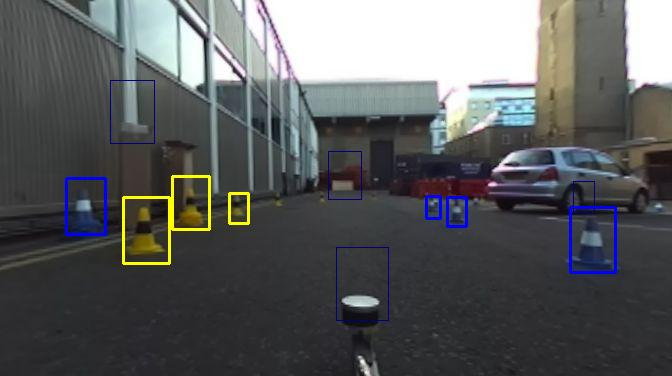
\includegraphics[width=0.49\linewidth]{img/single_lap/frame0134}
  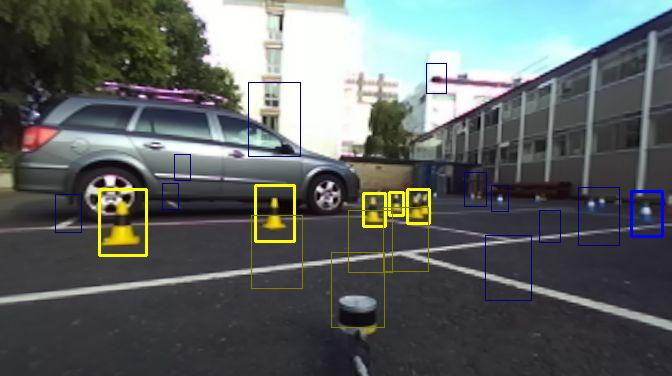
\includegraphics[width=0.49\linewidth]{img/single_lap/frame0212}
  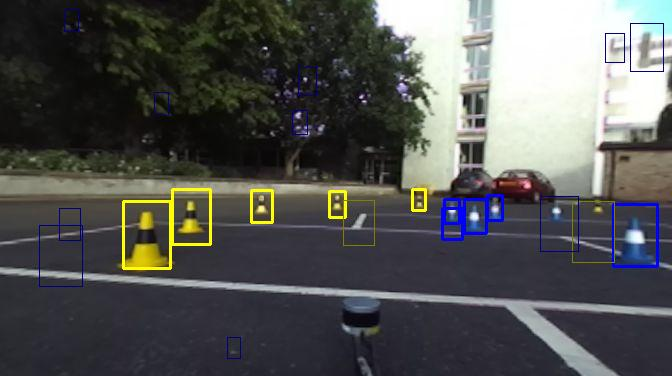
\includegraphics[width=0.49\linewidth]{img/single_lap/frame0253}
  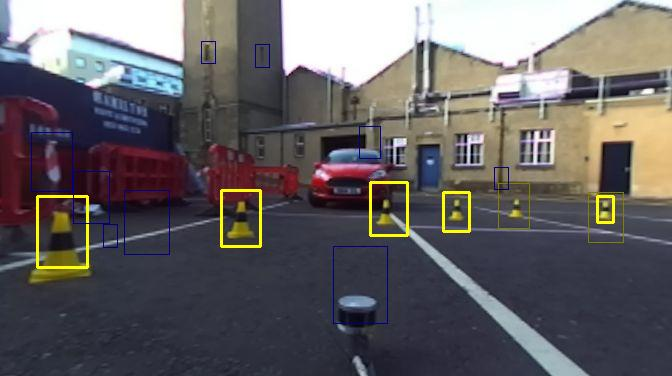
\includegraphics[width=0.49\linewidth]{img/single_lap/frame0175}
  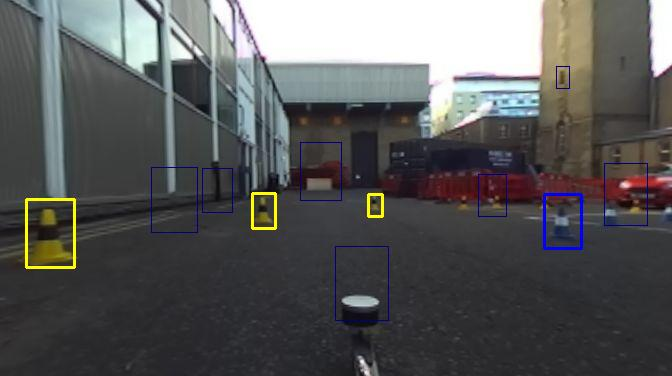
\includegraphics[width=0.49\linewidth]{img/single_lap/frame0152}
  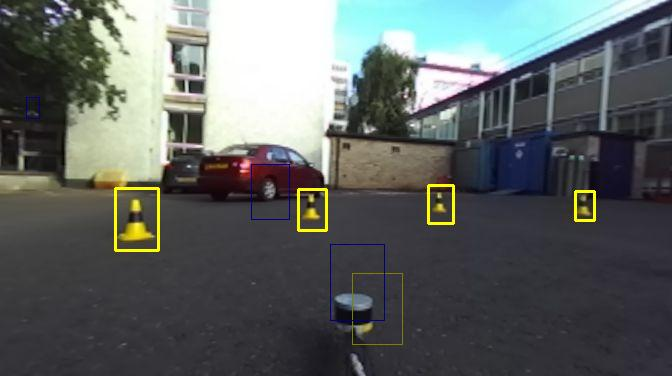
\includegraphics[width=0.49\linewidth]{img/single_lap/frame0278}\\[2ex]
  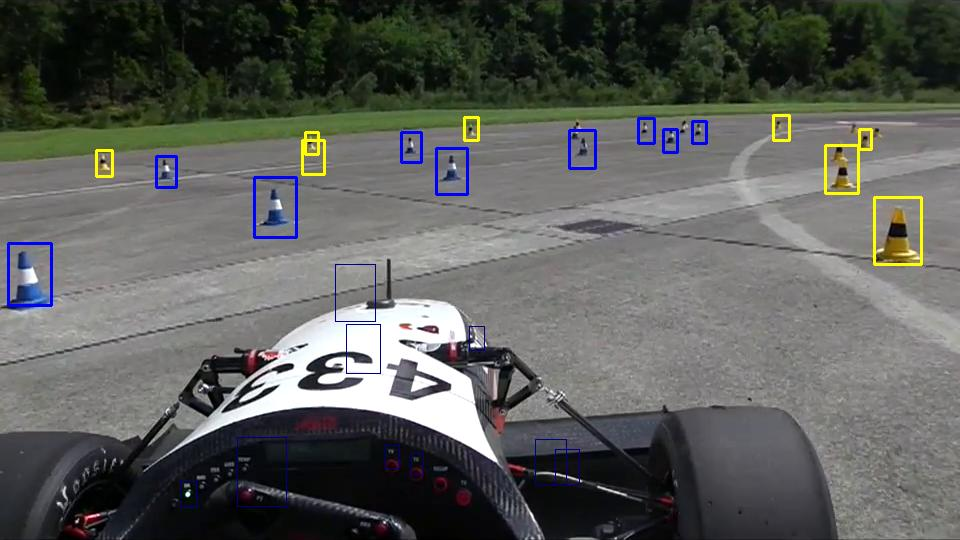
\includegraphics[width=0.49\linewidth]{img/amz/000513}
  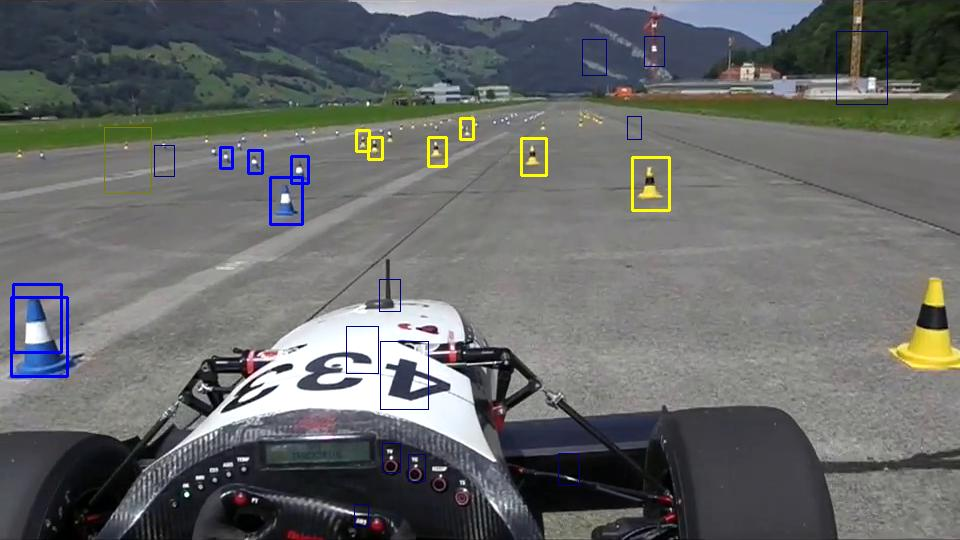
\includegraphics[width=0.49\linewidth]{img/amz/001345}
  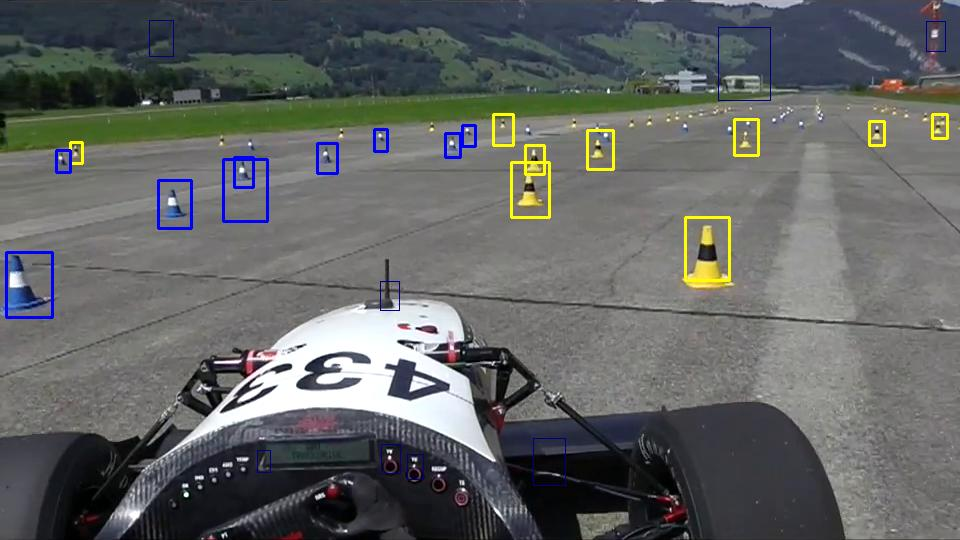
\includegraphics[width=0.49\linewidth]{img/amz/001617}
  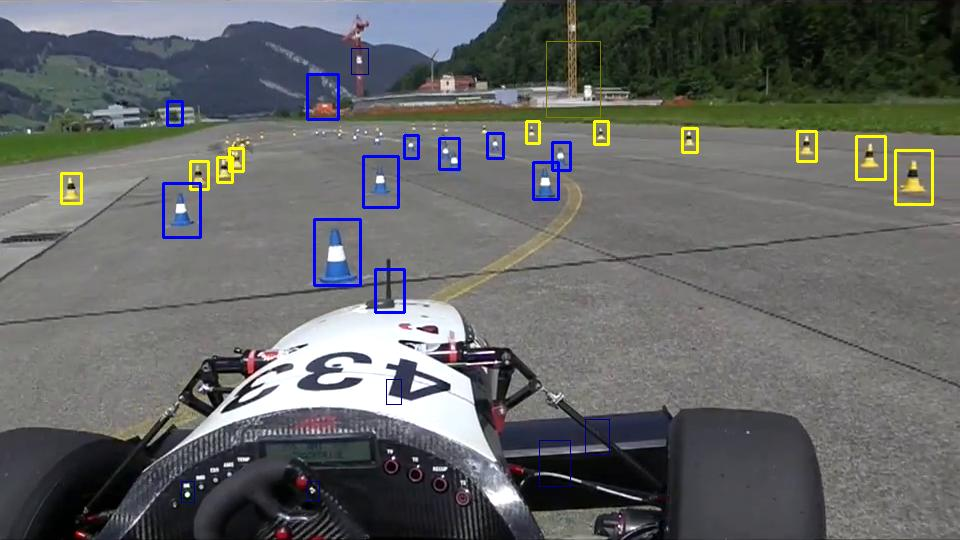
\includegraphics[width=0.49\linewidth]{img/amz/001941}
  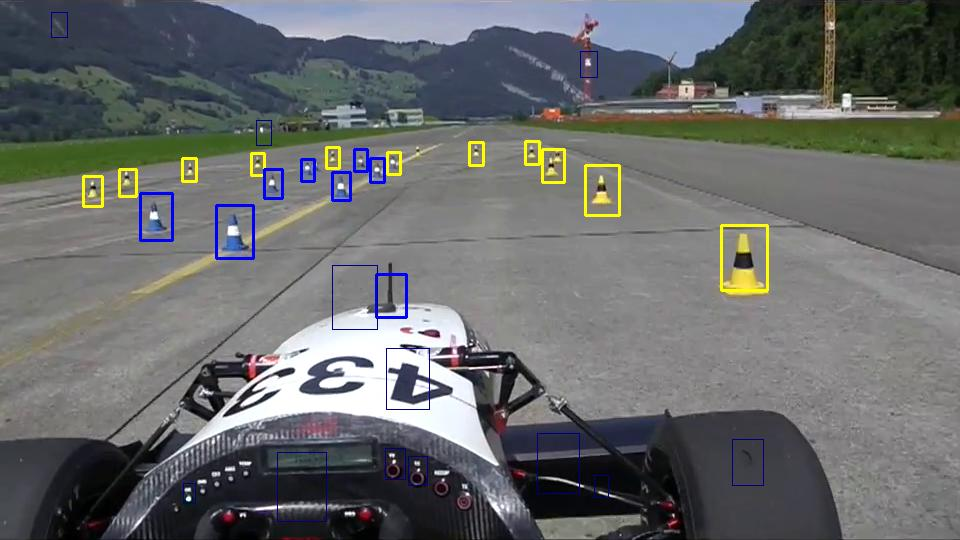
\includegraphics[width=0.49\linewidth]{img/amz/002317}
  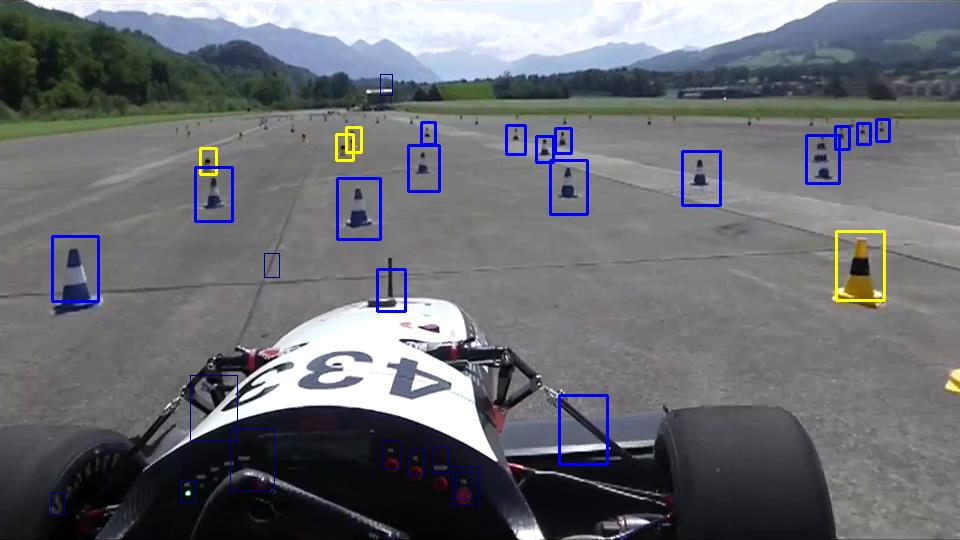
\includegraphics[width=0.49\linewidth]{img/amz/002605}\\
  \mycaption{Examples of cone detection. Thick lines indicate firm detections,
    thin lines indicate false detections discarded by the colour
    model. \textsl{Top:} StreetDrone data; \textsl{bottom:} AMZ data.}
  \label{fig:cones}
\end{figurehere}
\end{minipage}

\mysection{Path Planning}
We employ Hybrid A*~\cite{dolgov08} with Dubins path and Euclidean heuristics.

Path is composed of motion primitives subject to the following constraints:
\begin{itemize}
\item The distance travelled $d$ has to be enough to exit the cell:
  $d \ge \sqrt{2}\cdot s$ for a cell of size $s$.
  \item The curvature is restricted by the maximum vehicle steering angle $\alpha$.
\end{itemize}

  \begin{minipage}{\linewidth}
\begin{figurehere}
  \centering
  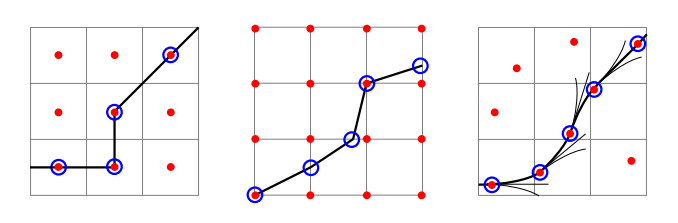
\includegraphics[width=1\linewidth]{img/comparison}
  \vspace{-2em}
  \mycaption{Comparison of search algorithms. Nodes are represented by the red
    dots. \emph{Left:} A*, \emph{centre:} D*, \emph{right:} hybrid-state
    A*. (From~Dolgov~\emph{et. al}~\cite{dolgov08})}
  \label{fig:comparison}
\end{figurehere}
\end{minipage}


\begin{minipage}{1.0\linewidth}
  \begin{figurehere}
    \centering 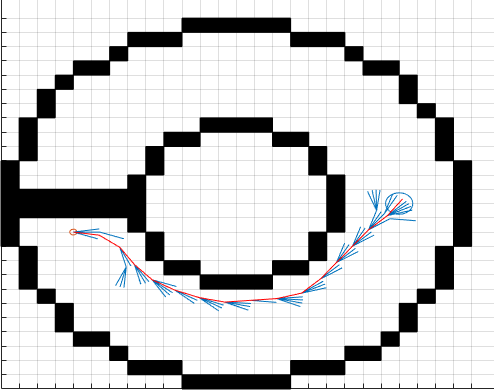
\includegraphics[width=0.49\linewidth]{img/half_cropped}
    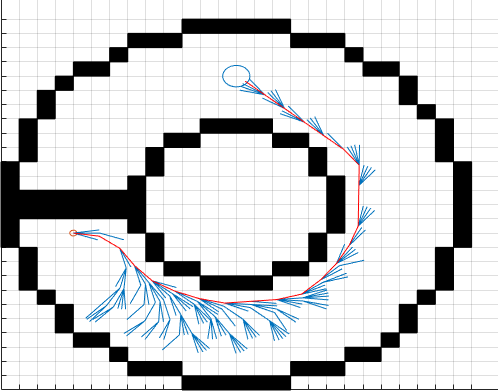
\includegraphics[width=0.49\linewidth]{img/three_quarters_cropped}\\
    % (a)\qquad\qquad\qquad\qquad\qquad\quad(b)\\
    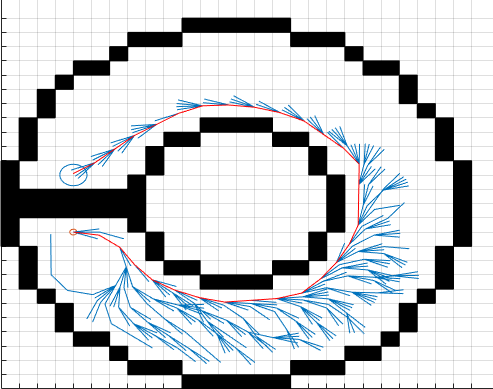
\includegraphics[width=0.49\linewidth]{img/full_cropped}
    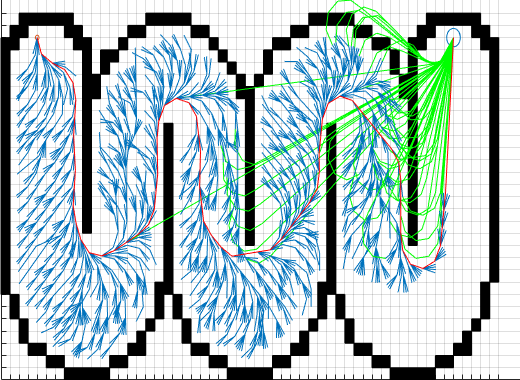
\includegraphics[width=0.49\linewidth]{img/snake_cropped}\\
    % (c)\qquad\qquad\qquad\qquad\qquad\quad(d)\\
    \raisebox{8ex}{\begin{minipage}{0.49\linewidth}
        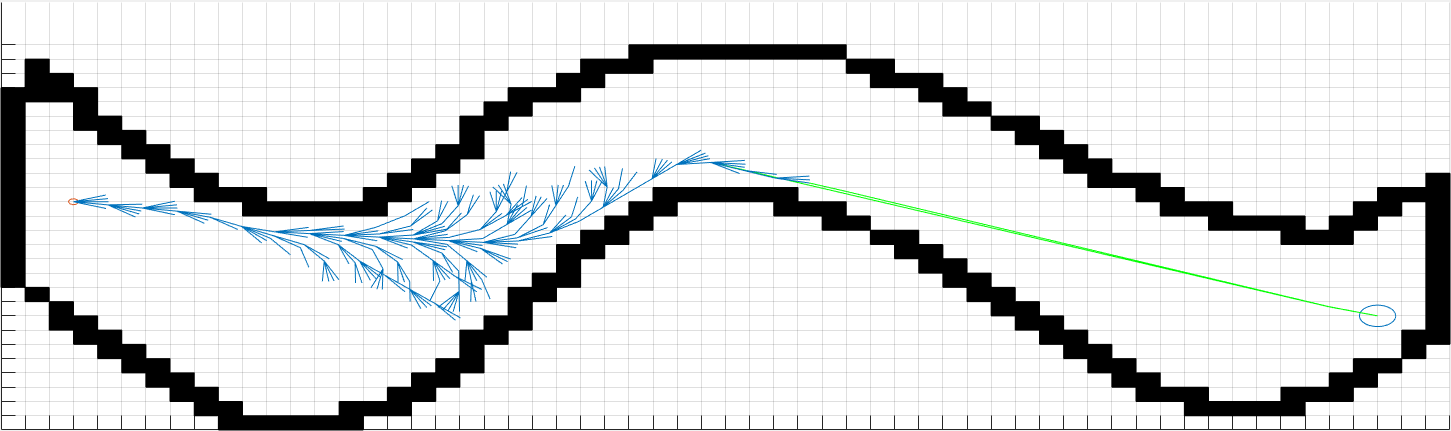
\includegraphics[width=1\linewidth]{img/long_snake_cropped}
        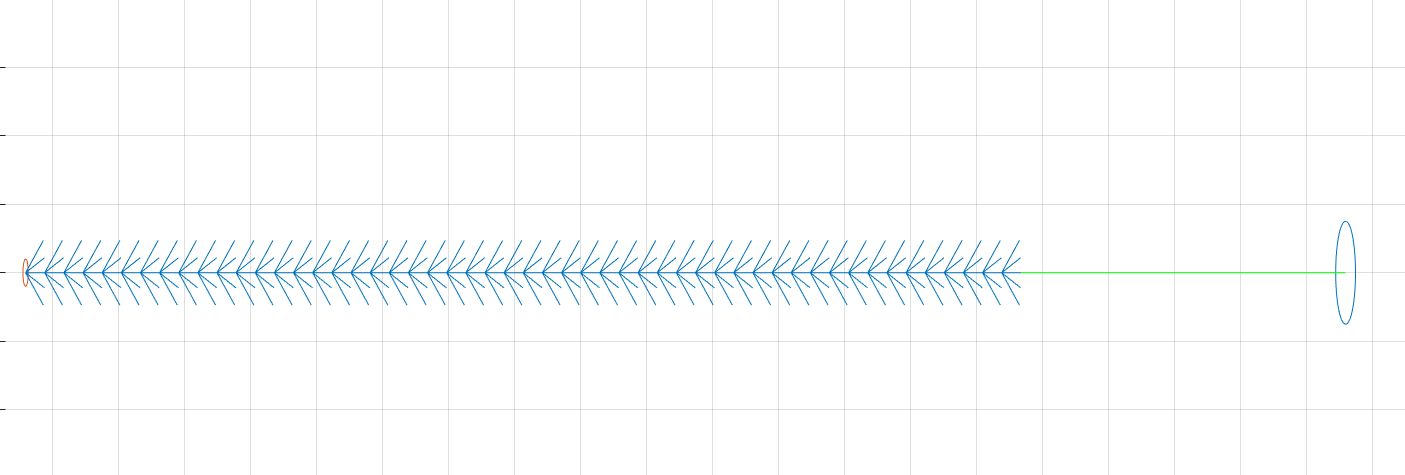
\includegraphics[width=1\linewidth]{img/trivial_cropped}
      \end{minipage}}
    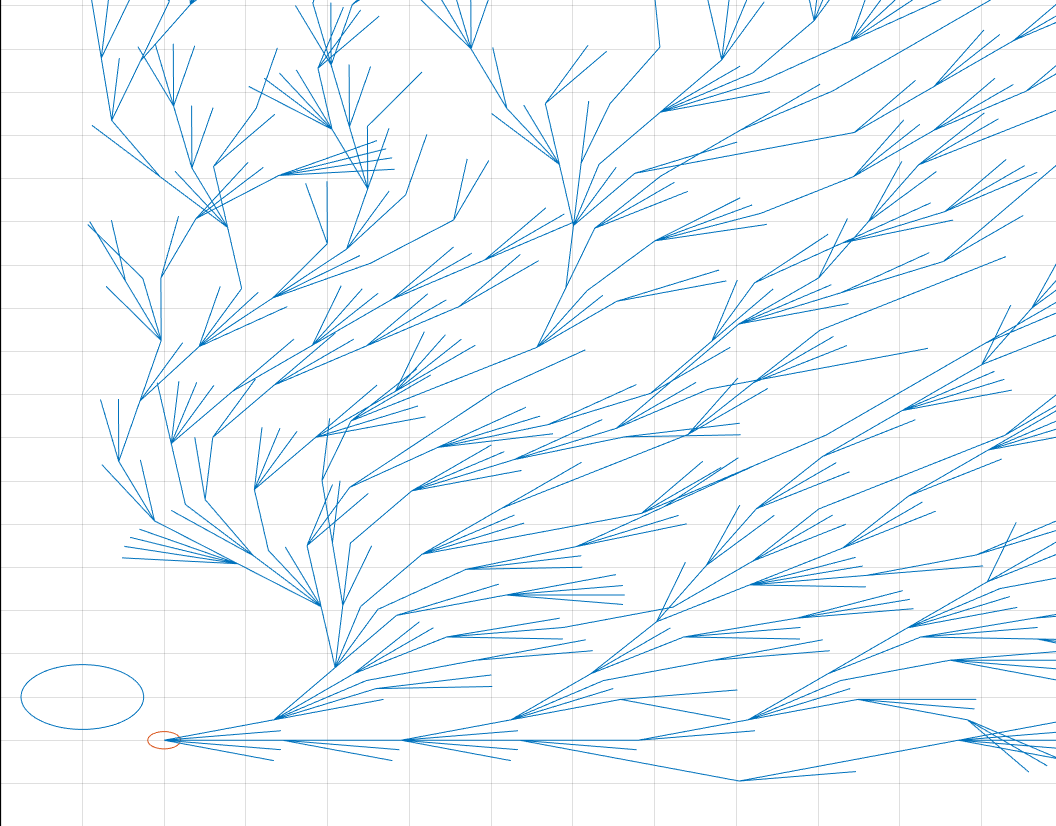
\includegraphics[width=0.49\linewidth]{img/empty_cropped}
    % (e)\qquad\qquad\qquad\qquad\qquad\quad(f)\\
    \label{fig:comparison}
  \end{figurehere}
\end{minipage}

\begin{figurehere}
  \centering
  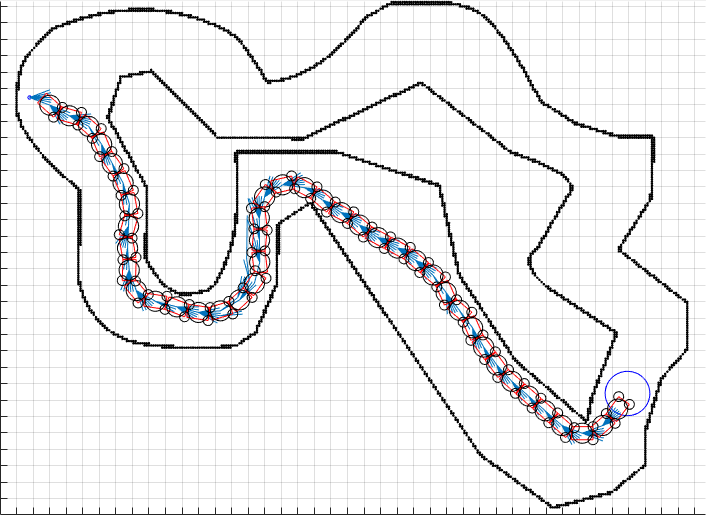
\includegraphics[width=0.49\linewidth]{img/new_collision_astar}
  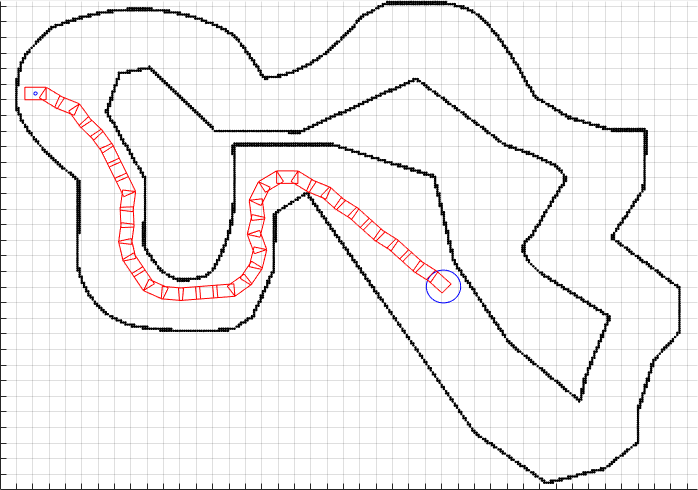
\includegraphics[width=0.49\linewidth]{img/new_solution_skeleton}
  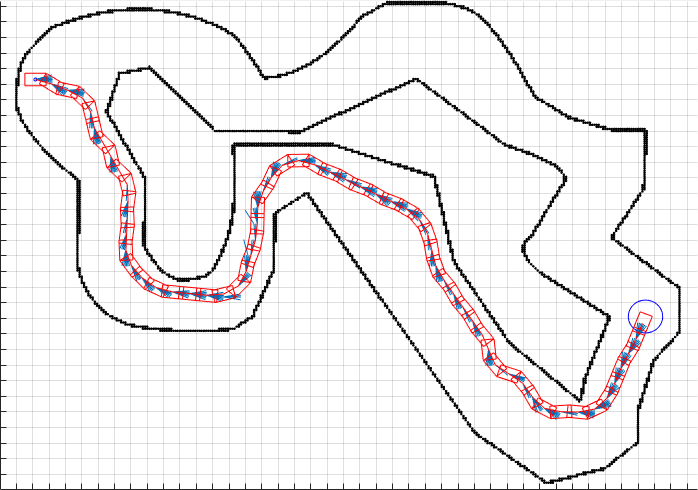
\includegraphics[width=0.49\linewidth]{img/new_long_astar_skeleton}
  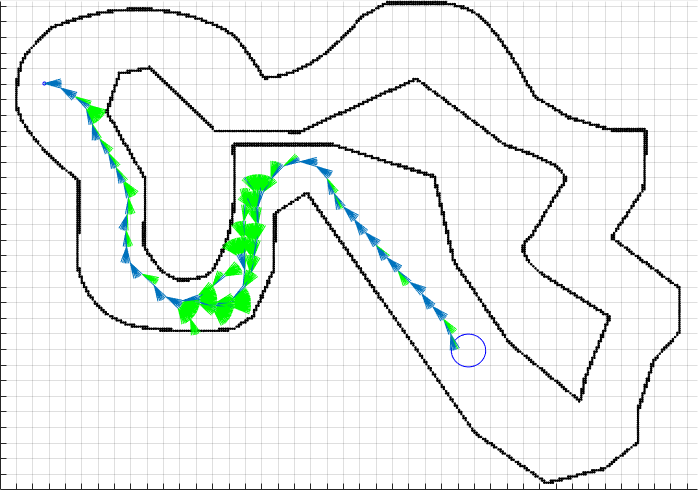
\includegraphics[width=0.49\linewidth]{img/new_astar_fullsearch}\\
  \mycaption{Illustration of motion planning with Hybrid A* and driveable
    motion primitives.}
\label{fig:collision_new}
\end{figurehere}
~\\[2ex]
\begin{figurehere}
  \centering
  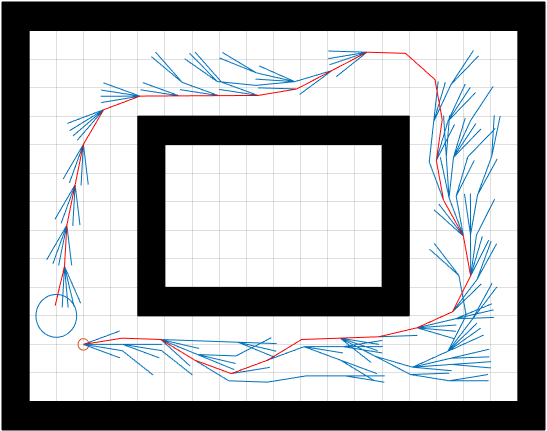
\includegraphics[width=0.49\linewidth]{img/euclidean1_cropped}
  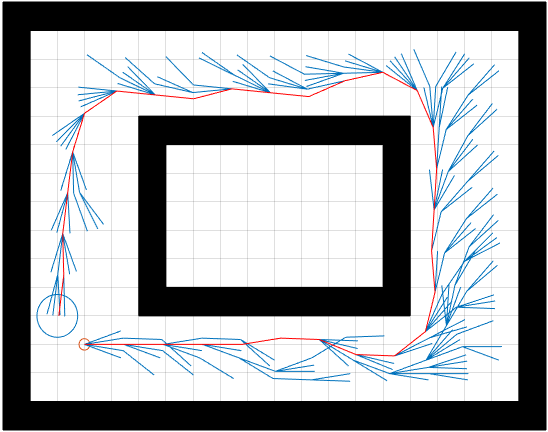
\includegraphics[width=0.49\linewidth]{img/euclidean2_cropped}
  \mycaption{The effect of introducing additional penalty for large steering
    angles to the Euclidean heuristic.}
  \label{fig:euclidean}
\end{figurehere}
Post-optimisation with a Nelder-Mean optimiser~\cite{press07}. Objective function~\cite{dolgov08}:
\begin{equation*}
  {\fontsize{25}{25}\selectfont% \small
  \begin{split}
  \mathrm{\min}\leftarrow w_{\rho}\sum_{i=1}^N\rho_d(x_i, y_i)+
  w_o\sum_{i=1}^N(|\vec{x}_i-\vec{o}_i|-d_{\mathrm{max}})^2+\\
  w_{\kappa}\sum_{i=1}^{N-1}\left(\frac{\Delta \phi_i}{|\Delta
      \vec{x}_i|} - \kappa_{\mathrm{max}} \right)^2+
  w_s\sum_{i=1}^{N-1}(\Delta\vec{x}_{i+1}-\Delta\vec{x}_i)^2,
\end{split}
  \label{eq:post}}
\end{equation*}
serves to improve smoothness and lengths of the solution.

\mysection{Simulation}
\begin{figurehere}
  \centering
  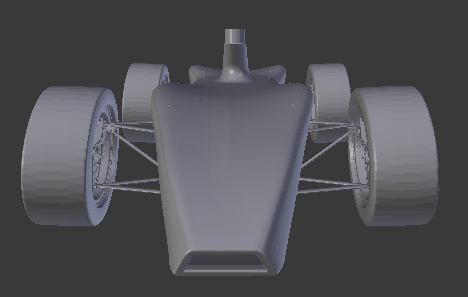
\includegraphics[height=0.18\linewidth]{img/model2}
  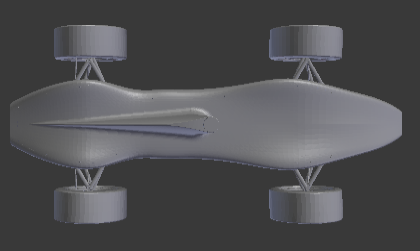
\includegraphics[height=0.18\linewidth]{img/model3}
  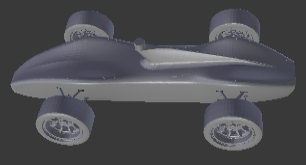
\includegraphics[height=0.18\linewidth]{img/model4}
  \mycaption{CAD models used in the simulation.}
  \label{fig:cad}
\end{figurehere}
\begin{minipage}{1.0\linewidth}
  \begin{figurehere}
    \centering 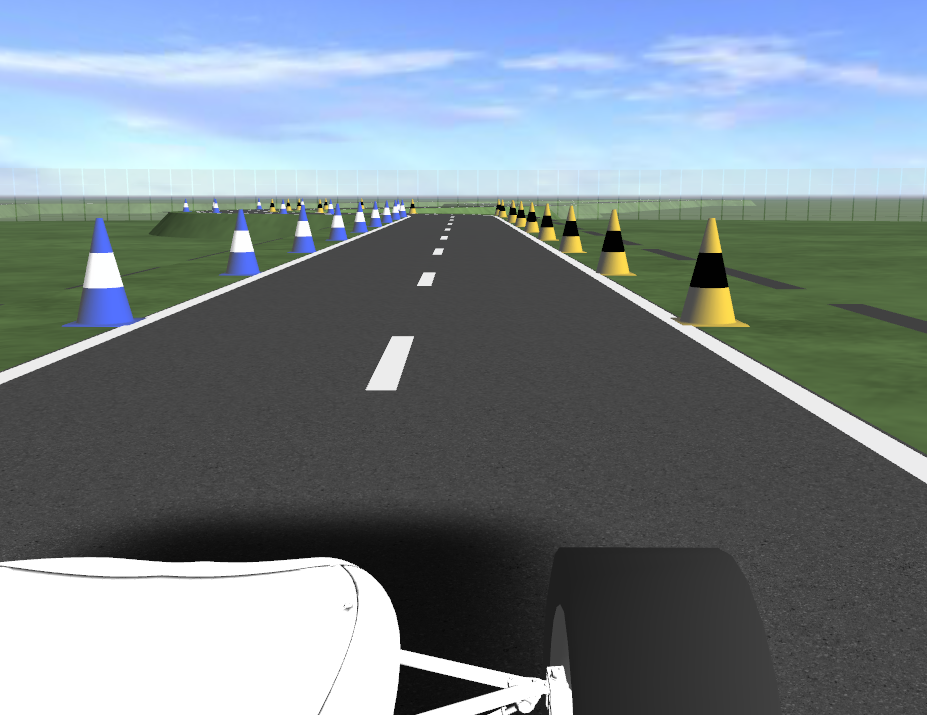
\includegraphics[width=0.49\linewidth]{img/ipg1_cropped}
    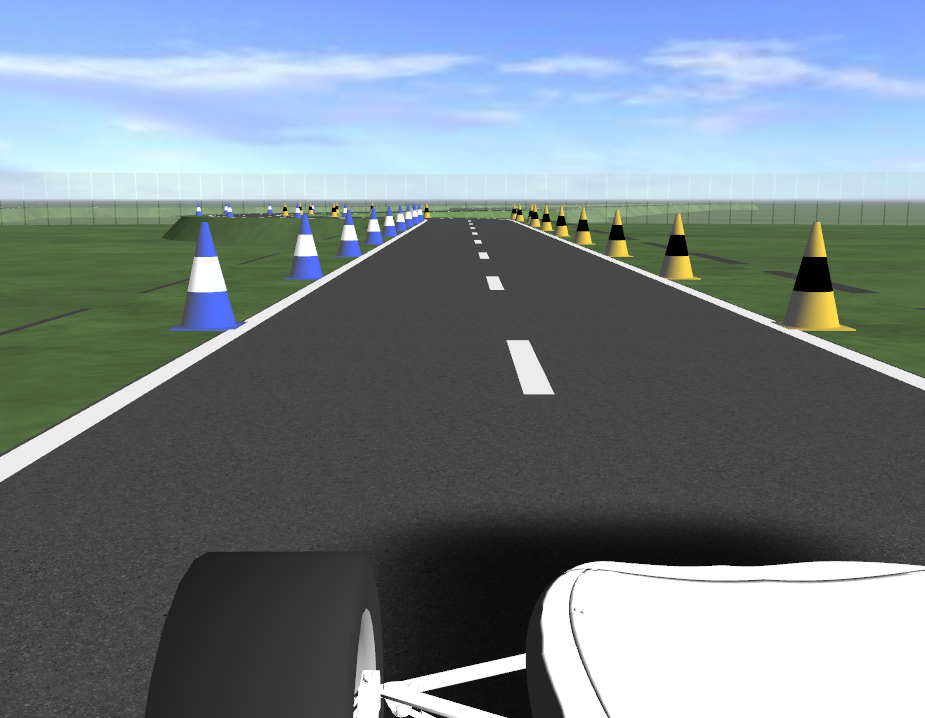
\includegraphics[width=0.49\linewidth]{img/ipg4_cropped}\\
    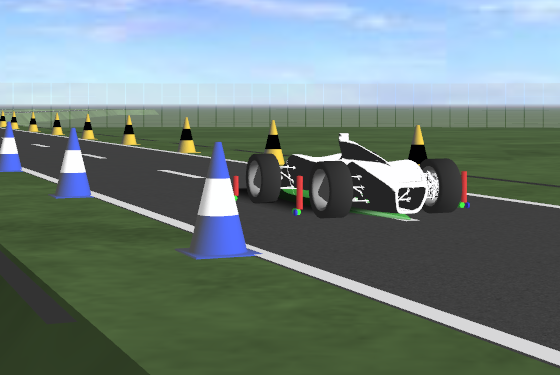
\includegraphics[width=0.49\linewidth]{img/ipg5_cropped}
    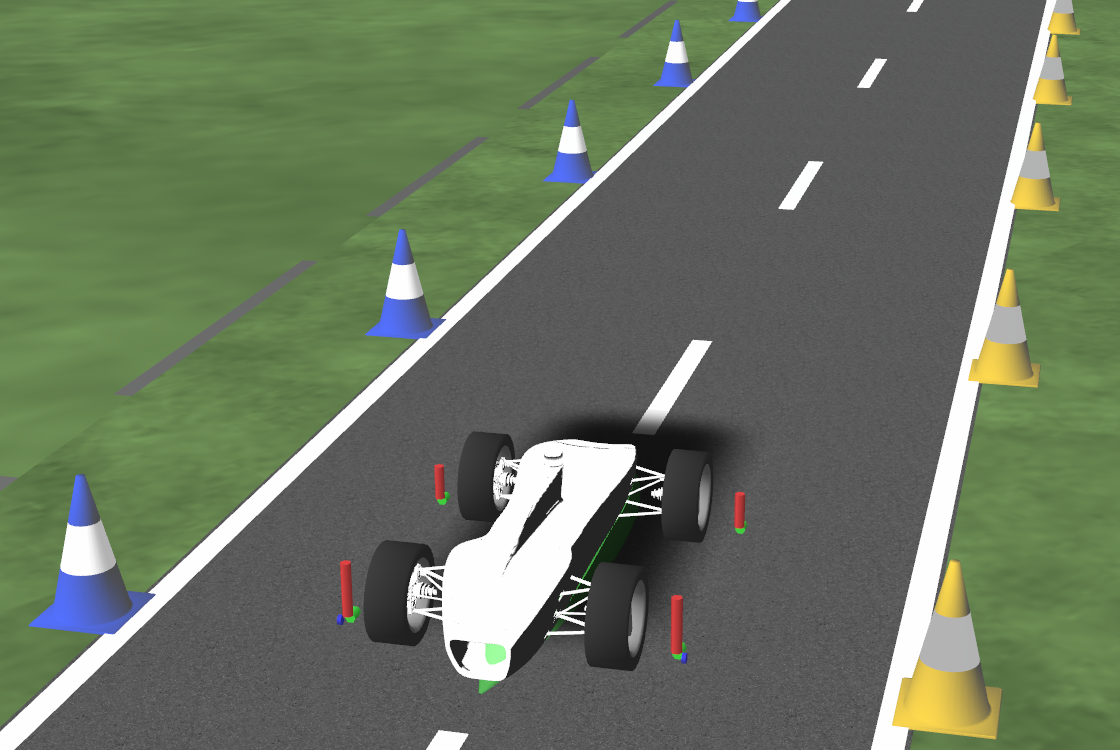
\includegraphics[width=0.49\linewidth]{img/ipg6_cropped}\\
    \mycaption{Camera
      views from the IPG CarMaker simulator.}
    \label{fig:ipg}
  \end{figurehere}
\end{minipage}
\begin{minipage}{1.0\linewidth}
  \begin{figurehere}
    \centering 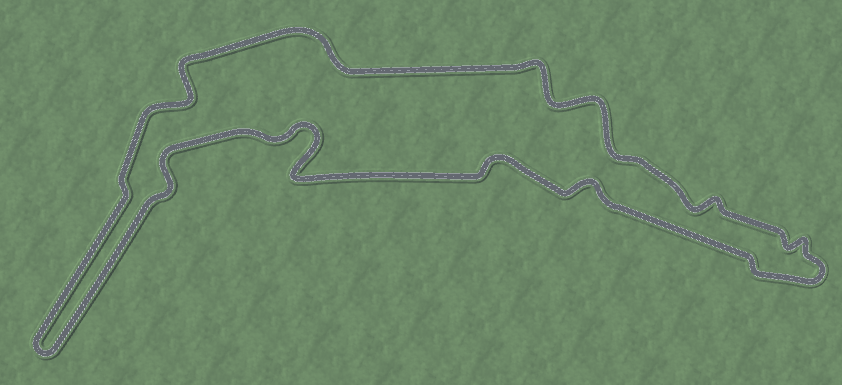
\includegraphics[width=0.8\linewidth]{img/track15_horiz}
    \mycaption{Silverstone FS 2015 track modeled in IPG.}
    \label{fig:silverstone}
  \end{figurehere}
\end{minipage}\\[2ex]
\begin{tablehere}
  \centering
  \scriptsize
  \begin{tabular}{llll}
    \toprule
    Parameter & Value & Parameter & Value\\
    \midrule
    Length & \textbf{1.170 m} & Height & \textbf{0.229 m}\\
               Body mass &
                                                                        \textbf{191.84 kg}&
                           Overall mass & \textbf{308.90 kg} \\
    Rotation (torsion) & 5000 Nm/deg & Rotation (bending) & 15000 Nm/deg\\
    Front wheel carrier mass & 1.67 kg & Back wheel carrier mass & 1.44 kg \\
                                                                           Wheel
                                                                           mass
                                                      & 8.71 kg &
                                                        Engine mount stiffness & 50000 N/m\\
    Engine mount damping & 500 Ns/m &
                                                                           Susp.
                                                                           spring
                                                                           stiffness
                                                      & 35000 N/m\\
    Front damping (push) & 2500 Ns/m & Front damping (pull) & 5000 Ns/m \\ Buffer
                                                                        stiffness
                                                                        (push)
                                                      & 5000 N/m &
    Buffer stiffness (pull) & 5000 N/m \\ Front stabilizer stiffness & 287 N/m &
                                                                              Rear
                                                                                stabilizer
                                                                                stiffness
                                                      & 191.9 N/m\\




                      Steering pinion angle & 100 rad/m & Motor power & 17 kW \\
                                                                               Motor torque & 55 Nm&
    Aerodynamic ref. area & 2 m$^2$\\ Aerodynamic ref. length & 1.3 m
                                          & &\\
        \bottomrule
  \end{tabular}
  \mycaption{Vehicle parameters in IPG CarMaker. In bold: measured from the
    platform vehicle, other parameters are estimated.}
  \label{tab:ipg}
\end{tablehere}
\mysection{Future Work}
\begin{itemize}
\item Develop reliable SLAM sub-system.
\item Optimise the trajectory
and the velocity profile jointly~\cite{xu12}.
\item Consider other sensors: IMU, LiDAR, a stereopair of cameras, and their fusion.
\item Investigate whether reinforcement learning~\cite{mnih15} can be
  applied to driverless racing control.
  \item Derive control heuristics by learning from a human driver.
  \item Develop a path following controller~\cite{ni17}.
    \item Model of drive-by-wire controls, such as
      throttle, steering, and braking-by-wire.
      \item Integration with ROS.
\end{itemize}
  % -------------------------------------------------------------------------
\mysection{Acknowledgements}
The authors would like to thank \mbox{MathWorks} for providing competition \mbox{MATLAB}
licenses and IPG Automotive for providing the IPG CarMaker simulator.\\[2ex]

\centerline{
\includegraphics[width=0.9\linewidth]{img/ipg}}
\centerline{
\includegraphics[width=0.9\linewidth]{img/mathworks_big}}
  \mysection{References}
  {
    \footnotesize
\bibliographystyle{IEEEtran}
\bibliography{adr}
  }
\end{multicols}
\end{document}

%%% Local Variables: 
%%% coding: utf-8
%%% mode: latex
%%% TeX-engine: xetex
%%% End: 
